\documentclass{article} % For LaTeX2e
\usepackage{nips13submit_e,times}
\usepackage{amsmath,amssymb,amsthm}
\usepackage{url}
\usepackage[pdftex]{graphicx}
\usepackage{subfig}
\usepackage{wrapfig}
\usepackage{hyperref}


\title{Predicting Mental Functions from Brain Activations}


\author{
Madhura Parikh\thanks{Authors contributed equally}\\
Department of Computer Science\\
University of Texas, Austin\\
\texttt{mparikh@cs.utexas.edu} \\
\And
Subhashini Venugopalan\footnotemark[1] \\
Department of Computer Science\\
University of Texas, Austin\\
\texttt{vsub@cs.utexas.edu} \\
}

% The \author macro works with any number of authors. There are two commands
% used to separate the names and addresses of multiple authors: \And and \AND.
%
% Using \And between authors leaves it to \LaTeX{} to determine where to break
% the lines. Using \AND forces a linebreak at that point. So, if \LaTeX{}
% puts 3 of 4 authors names on the first line, and the last on the second
% line, try using \AND instead of \And before the third author name.

\newcommand{\fix}{\marginpar{FIX}}
\newcommand{\new}{\marginpar{NEW}}

%\nipsfinalcopy % Uncomment for camera-ready version

\begin{document}


\maketitle

\begin{abstract}
Over the past few decades neuroscientists have studied brain images from EEG/MEG, fMRI and other sources to identify associations between psychological tasks and activity in brain regions~\cite{PMSKBY12}.
Although these studies have led to large amounts of literature and several discoveries of cognitive functions associated with certain brain regions (or networks) the mapping between functions to brain regions and vice-versa still remains largely unclear. For the purposes of this project, we look at enhancing a new automated framework NeuroSynth~\cite{yarkoni2011large}  that combines text-mining and machine learning techniques to generate probabilistic mappings between cognitive and neural states. Starting from their Naive Bayes classifier, we apply more sophisticated binary classifiers to the problem and also consider multi-label predictions and transfer-learning(?).
\end{abstract}

\section{Introduction}

\subsection{Our Contribution}

\section{Related Work}

\section{Methods}
 \paragraph{Notation}: We denote matrices by boldface capital letters $\mathbf{X}$ and vectors by bold-face lower case letters $\mathbf{x}$. The set of real valued $D$ dimensional vectors are denoted by $\mathbb{R}^D$. The set of (target) labels are denoted by the letter $\mathcal{L}$, and $|\mathcal{L}|$ denotes the cardinality of the set of labels.

Our input data consists of brain volume images. We denote by $\mathbf{x}_n$ the $n^{th}$ brain volume with voxels collected in a real valued $D$ dimensional vector. The total number of brain volumes is represented by $N$. Each brain volume is associated with a set of labels $\mathcal{L}_n = {l_1, \ldots, l_K}$ chosen from the full set of possible target labels $\mathcal{T} = \cup_{n=1,\ldots,N} \mathcal{L}_n$ with $|\mathcal{L}|=L$.

We approach the task of predicting brain functions as a classification task and address it using the following techniques:
 \subsection{Single Label Prediction}
  As a first step to measure the feasibility of the task we consider the task of predicting one of two labels for each brain volume. The single label prediction learns a mapping $f\ :\ \mathbf{x}_n \rightarrow \mathcal{L}_n$, such that $|\mathcal{L}_n|=1$ for all $n$, where $|\mathcal{T}| =| \cup \mathcal{L}_n| = 2$. This essentially learns a simple binary classifier for all pairs of labels. Each classifier is trained and tested on an appropriate subset of the data where the labels for the brain volume are unique. We experimented with the following binary classifiers:
  \begin{description}
  \item[Naive-Bayes] We built pairwise naive-bayes classifiers as a baseline to replicate the results presented in~\cite{yarkoni2011large}.
  \item[Logistic Regression] An $l_1$ regularized logistic regression was our next model of choice for a more powerful classifier.
  \item[Linear SVM] We use a linear SVM which scales well with the size of our features. The hyperparameter C is optimized by a grid search in the space $C = \{1, 10, 100, 1000\}$.
  \item[Ensemble] We finally build an ensemble of the above three classifiers and consider the label that is the majority in the output of the above three classifiers.
  \end{description}
\begin{figure}[ht]
\vspace{-0.5cm}
\centering
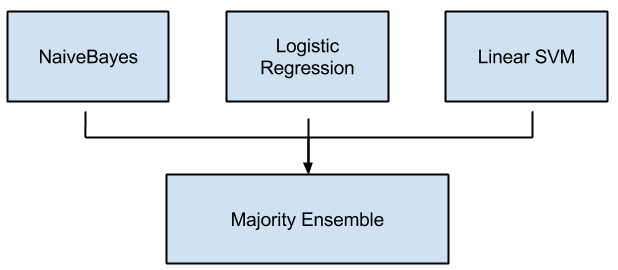
\includegraphics[scale=0.5]{./figs/single_pairwise.png}
\caption{We use naive-bayes, logistic regression, SVMs and a majority ensemble for pairwise binary classification of the labels.}
\end{figure}

 \subsection{Multi-Label Prediction} \label{subsec:method_multi}
Our next approach is to perform multilabel classification to predict multiple functions for a given brain volume. This learns a mapping $f\ :\ \mathbf{x}_n \rightarrow \mathcal{L}_n$, over the full set of labels (where $|\mathcal{L}_n| \geq 1$)  and $|\mathcal{T}| =| \cup \mathcal{L}_n|$. \cite{zhang2013review} suggests several methods to perform multilabel classification which include label projection, label ranking and label decomposition. We prefer the label decomposition method for it's ease of interpretation. In particular we choose the \textit{One-vs-All} decomposition approach. This method learns multiple binary classifiers ($|\mathcal{T}|$ to be precise), one for each label to predict the presence/absence of that label. Our experiments used the following binary classifiers for the multi-label prediction task:
  \begin{description}
  \item[Naive-Bayes] We built pairwise naive-bayes classifiers as a baseline to replicate the results presented in~\cite{yarkoni2011large}.
  \item[Logistic Regression] We build two models here. The first with $l_1$ or \textit{lasso} regularization and the other with $l_2$  or \textit{ridge} regularization. 
  \item[Linear SVM] In a manner similar to our single label prediction, we use a linear SVM by setting the hyperparameter C via a grid search in the space $C = \{1, 10, 100, 1000\}$.
  \item[Ward Clustering] Since the number of features in our data is extremely large, we do a dimensionality reduction of the features by first performing ward clustering [citation] and then mapping the points to different clusters. The number of clusters is 5000. We then apply a logistic regression classifier with $l_1$ regularization on the reduced data.
  \item[Unique train] Since our data is quite sparse and there's a high possibility of noise in data with multiple labels, we build what we call a unique train model based on logistic regression. In the unique train model, we identify all brain volumes with a single unique label, and train a classifier for each label using only this data. During test, we use the One-vs-All approach to test on multilabel brain volumes.
  \item[All ones] Another baseline we consider is the all ones baseline, which predicts ones for all labels on all input data points. Such a manipulation will give result in $100\%$ recall for the multilabel task, but very low precision values.
  \end{description}
In addition to the above, we did experiment with PCA and $k$-nearest neighbours for $k \in \{2,3,4\}$ but the models were not trained similarly or performed extremely poorly and hence we do not report results for these.
\begin{figure}[ht]
\vspace{-0.5cm}
\centering
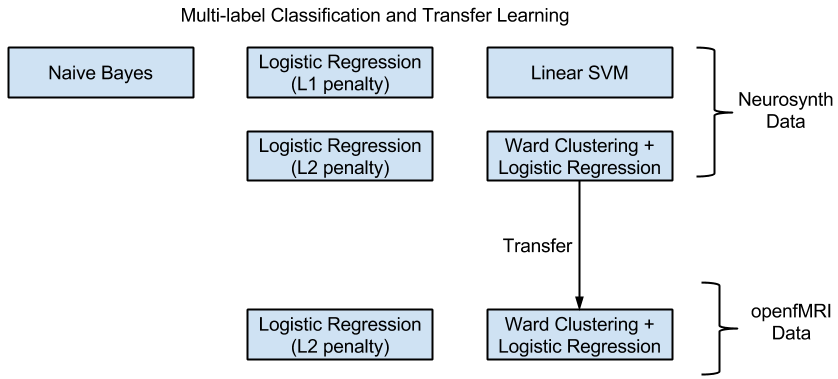
\includegraphics[scale=0.5]{./figs/multilabel_transfer.png}
\caption{We experiment several classifiers for the multilabel task. We pick our best performing models, namely logistic regression with $l_2$ penalty and the ward clustering based models and evaluate their performance on the openfMRI data. }
\end{figure}

 \subsection{Transfer Learning}
 As mentioned in Section~\ref{sec:neurosynth_framework}, one of the main purposes of this particular synthesis method for predicting brain functions is to be able to transfer the models from the synthesis domain to the real openfMRI domain. Based on the mapping functions that we learned in Section~\ref{subsec:method_multi} we want to apply the same function or a small modification of the function to new studies. That is, apply the mapping $f\ :\ \mathbf{x}_n \rightarrow \mathcal{L}_n$, to $\mathbf{x}'_n$ where ($\mathbf{x}'_n \notin \mathbf{X}$). In fact, our features $\mathbf{x}'_n$ are different both in dimension and constitution (the elements are continuous real valued data unlike the binary synthesis data). More details about the pre-processing is mentioned in Section~\ref{subsec:preprocessing}. In addition, we are interested in a predicting a different set of labels or functions, as constrained by the availability of data in the new domain. In effect, the transfer learning is attempting to learn $f'\ :\ \mathbf{x}'_n \rightarrow \mathcal{L}_n$. We experiment with the following methods here:
  \begin{description}
  \item[Ward Clustering] We reuse the ward clustering model that we learn previously by first performing ward clustering [citation] on the data in the synthesized domain to cluster and map the points to different clusters. We then train an $l_2$ regularized logistic regression \textit{One-vs-All} classifier on the data. Next we reapply the same clustering transformation to the openfMRI data and use the logistic classifier to predict the labels. The number of clusters is 5000.
  \item[Logistic Regression] For the sake of comparison we train an $l_2$ regularized logistic regression model directly on the openfMRI data.
  \end{description}

\section{Data}

\subsection{Preprocessing}

\section{Experimental Results}
Our experiments for single and multilabel prediction tasks were performed on data available in the neurosynth~\footnote{\protect \url{www.neurosynth.org}} tool. After preprocessing and filtering our inpput feature matrix  $\mathbf{X}$ is of dimension $5067 \times 228,453$, the target label matrix $\mathbf{Y}$ is of dimension $5067 \times 23$. The transfer learning component is tested on data from the openfMRI~\footnote{\protect \url{https://openfmri.org}} project with feature dimensions $\mathbf{X}'$ ($479 \times 174,264$) and targer label matrix $\mathbf{Y}'$ of dimensions $479 \times 19$.

Data samples size (4000). We use 10 fold cross validation to evaluate all our models unless otherwise indicated. We evaluate the performance of our models on the metrics such as \textit{accuracy, precision, recall, hamming loss, F1 score} which are frequently applied to this task.
\begin{align*}
% \text{Accuracy} &= & \text{Hamming loss}&= \\
 \text{Accuracy} &= 
\end{align*}

 \subsection{Single Label Prediction}
 We present the accuracies of the pairwise single label predictions using all our approaches in the heat maps below.
\begin{figure}[ht]
\vspace{-0.5cm}
\centering
\subfloat[Naive Bayes]{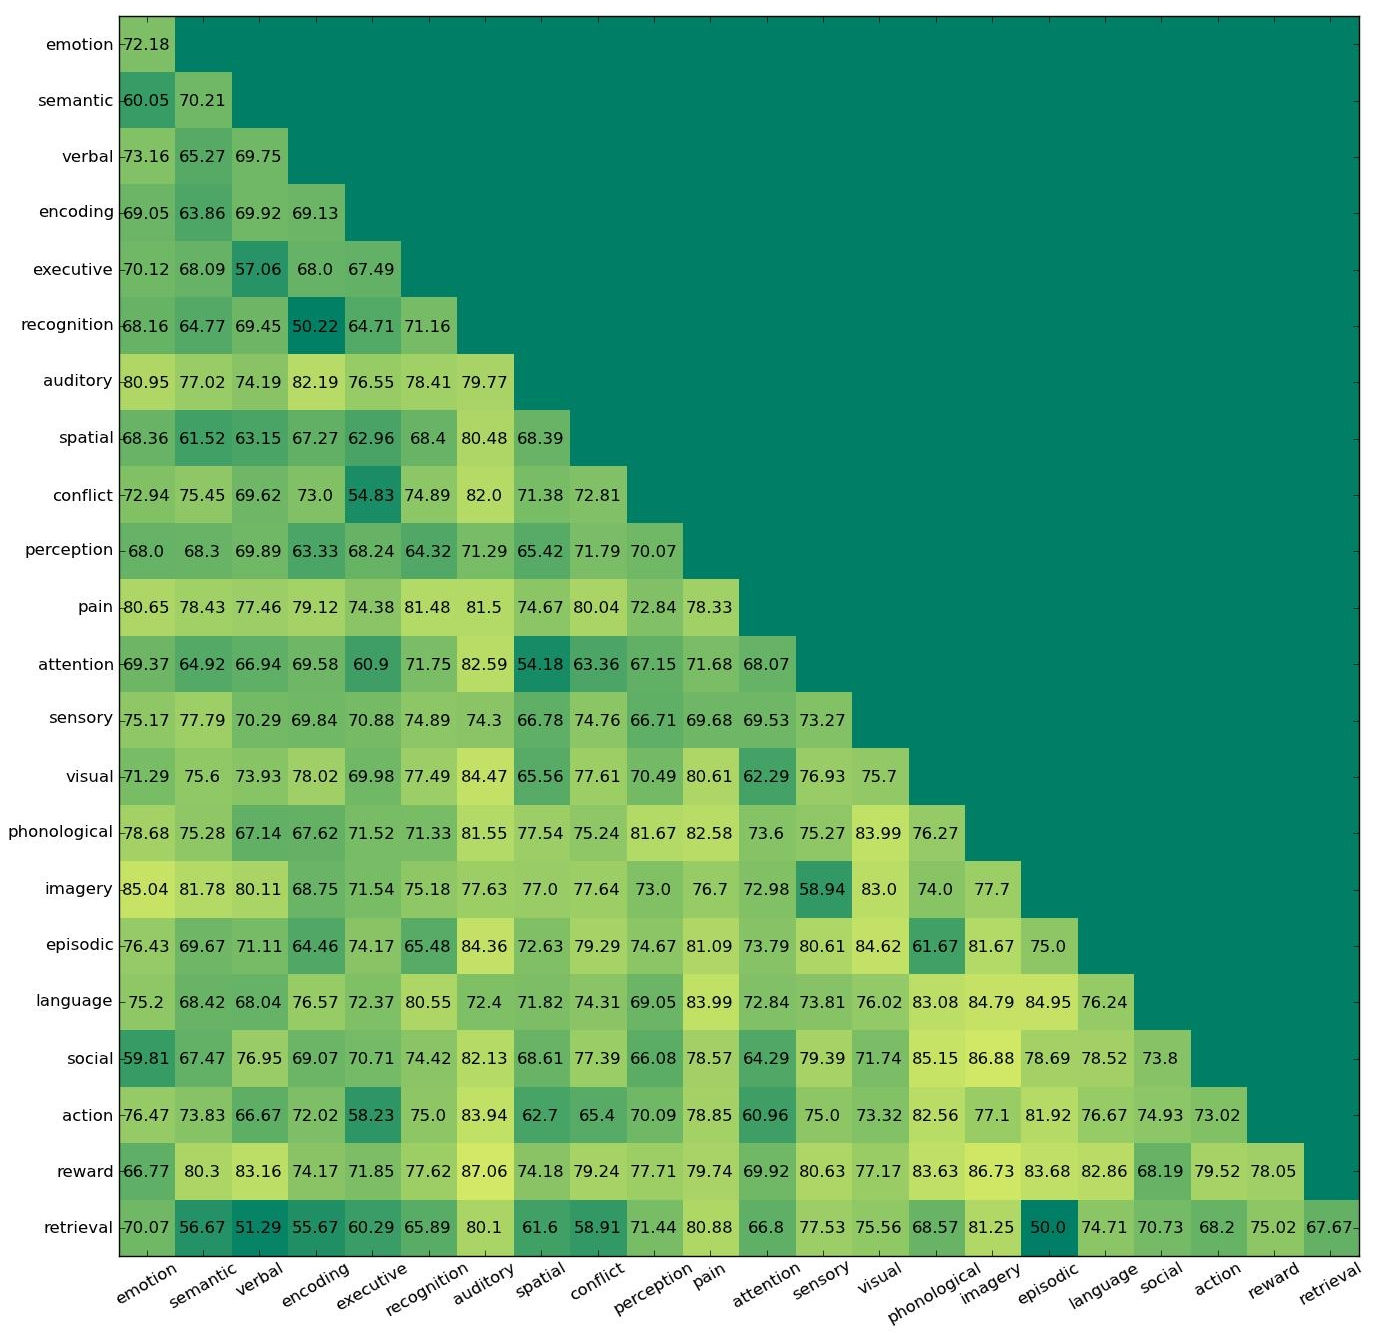
\includegraphics[width=12cm]{./figs/nb_confmat.jpg}} \\
\subfloat[Logistic Regression]{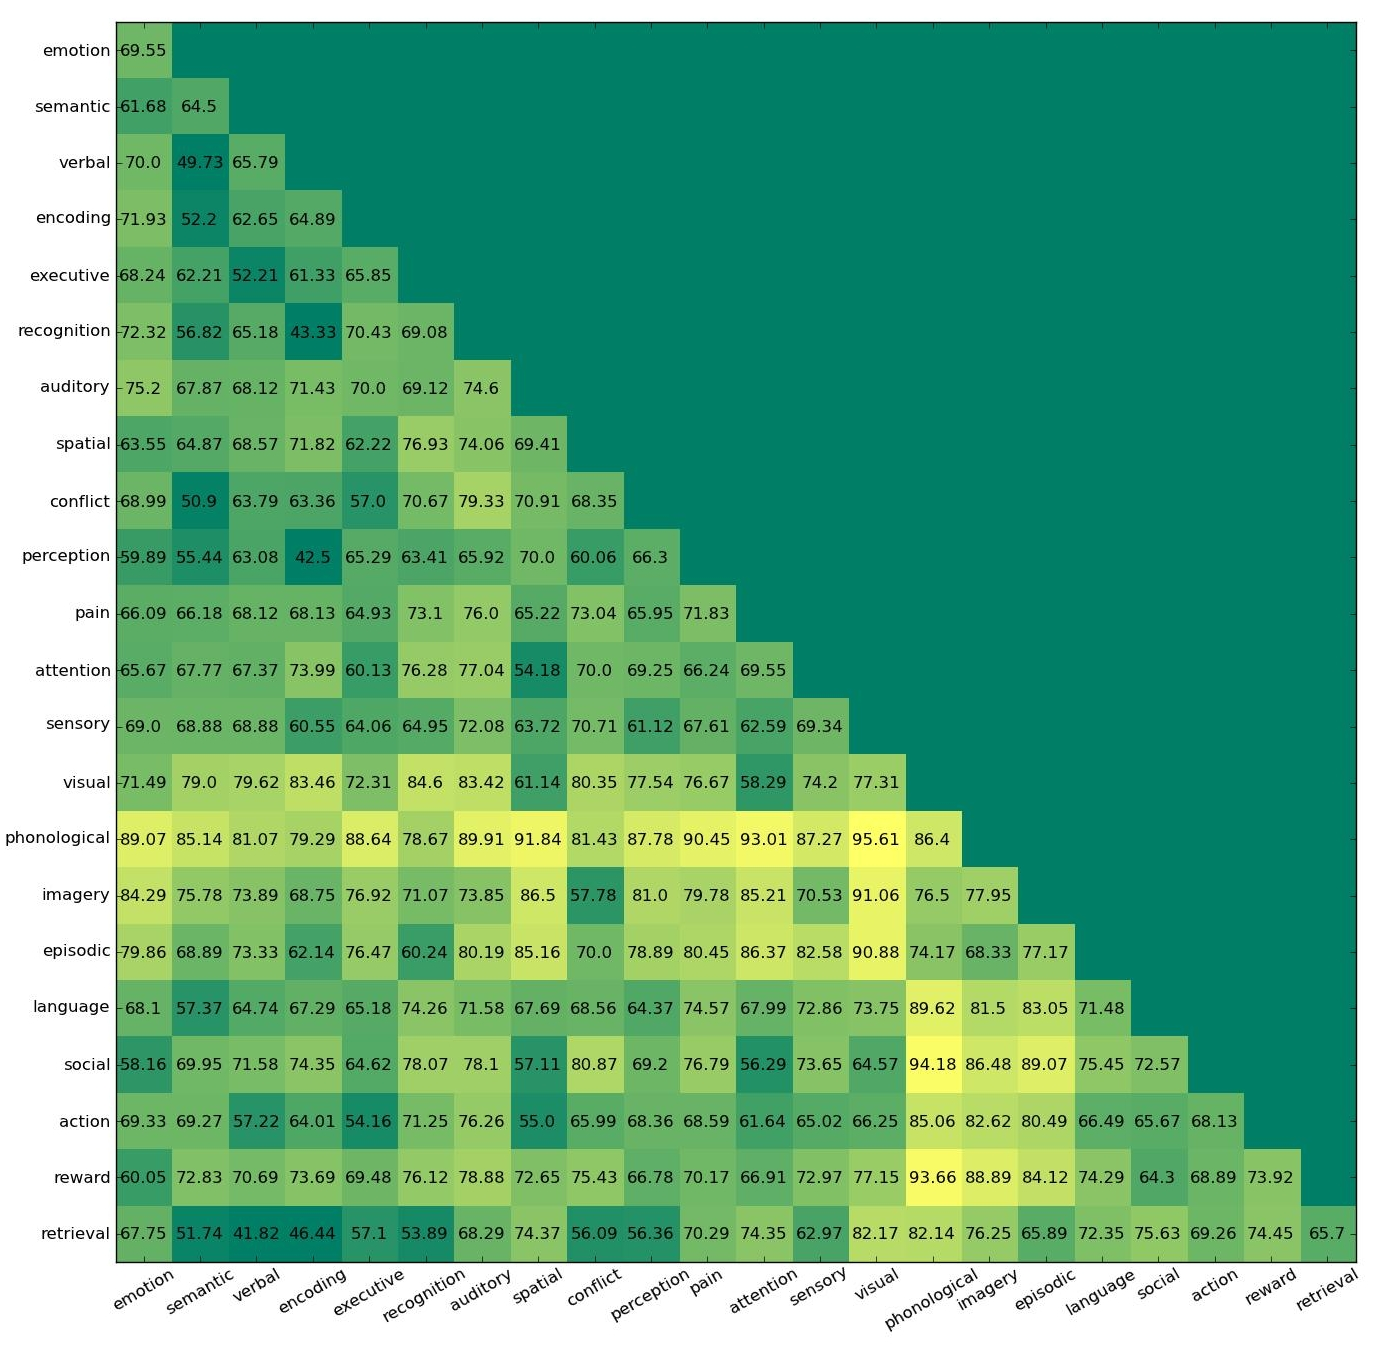
\includegraphics[width=12cm]{./figs/log_confmat.jpg}}
\caption{Pairwise binary classification accuracy for single label prediction}
\label{fig:singlelab1}
\end{figure}
\begin{figure}[ht]
\vspace{-0.5cm}
\centering
\subfloat[Linear SVM]{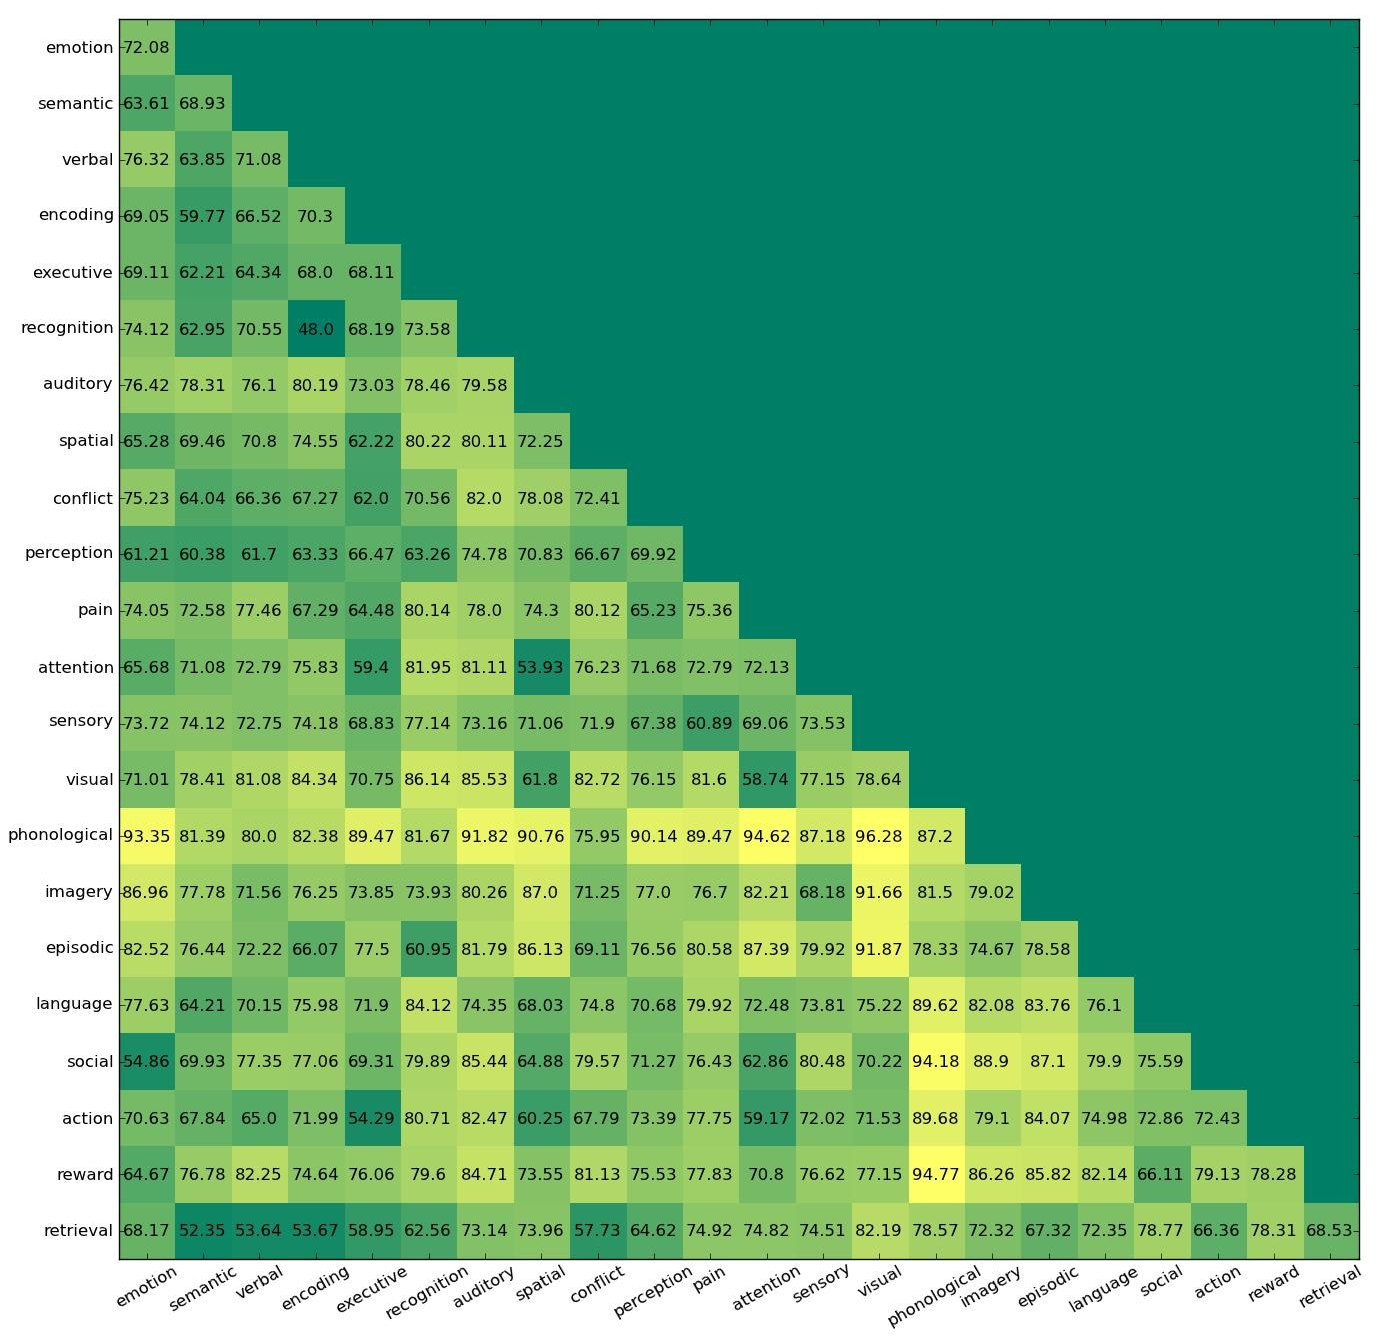
\includegraphics[width=12cm]{./figs/svm_confmat.jpg}} \\
\subfloat[Ensemble of naive bayes, logistic regression and SVM]{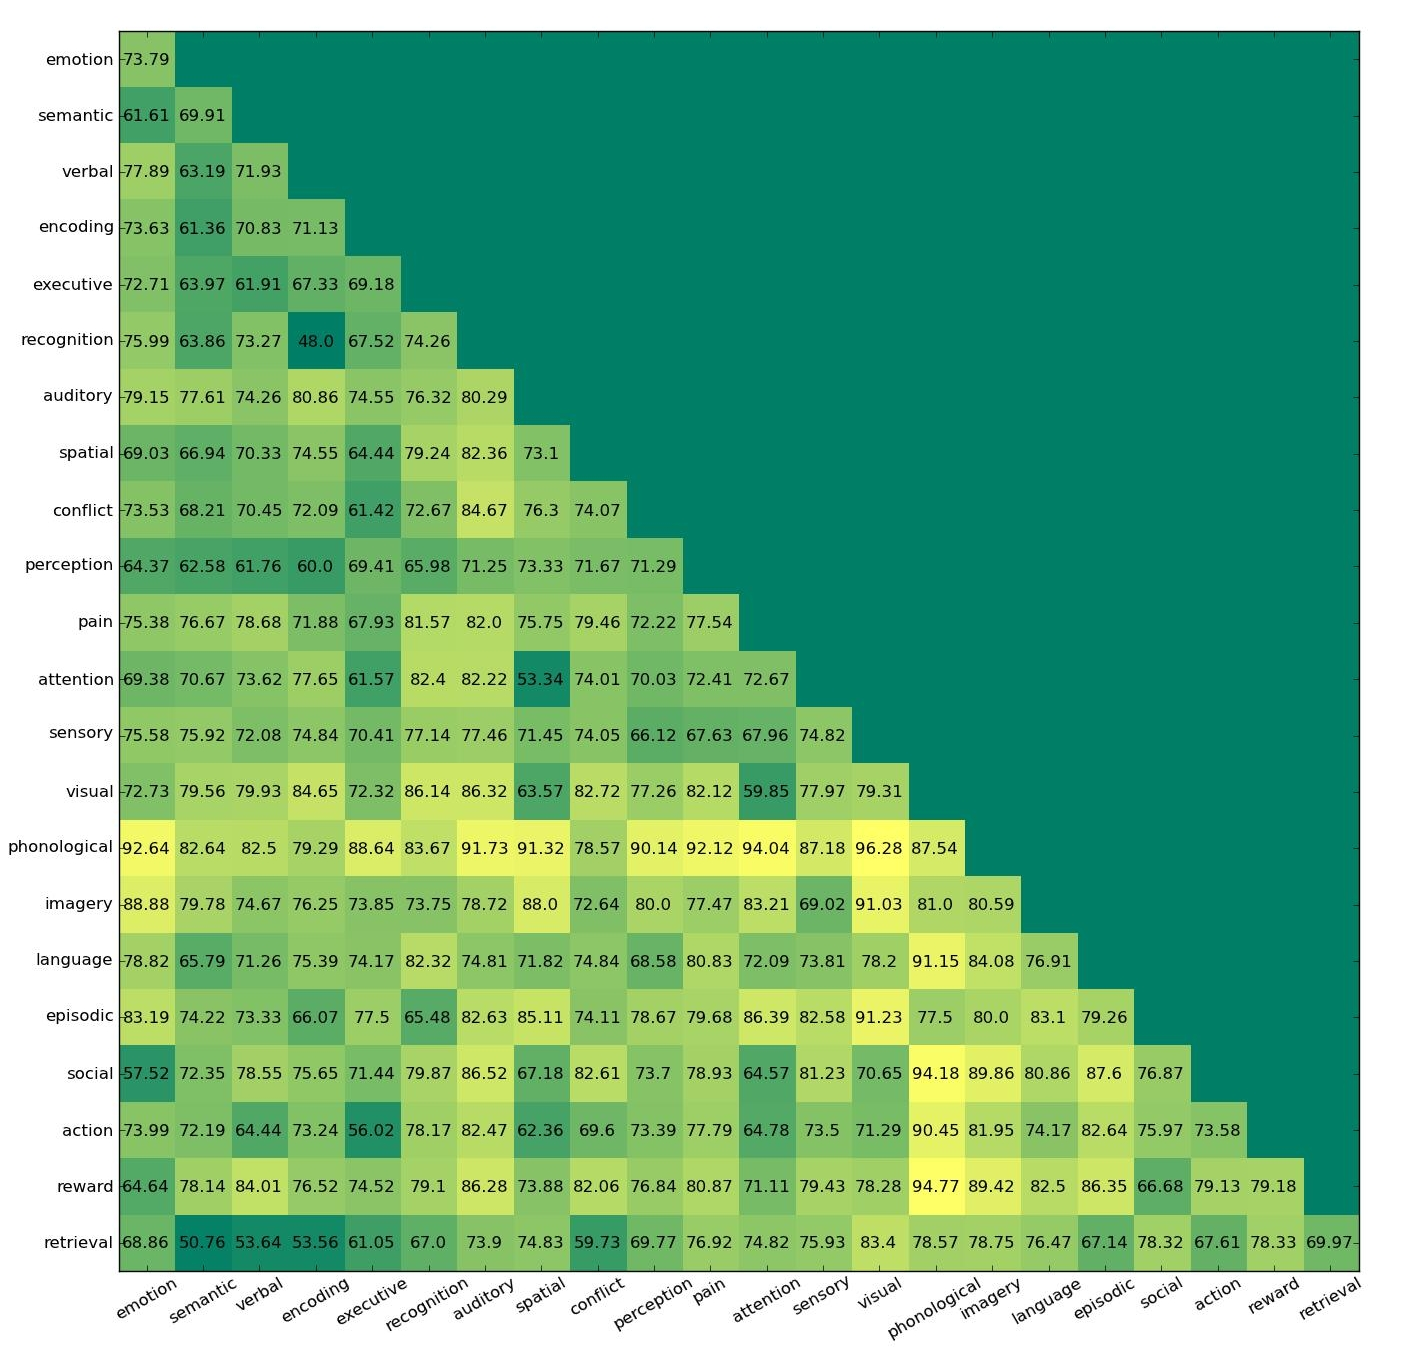
\includegraphics[width=12cm]{./figs/ensemble_confmat.jpg}}
\caption{Pairwise binary classification accuracy for single label prediction}
\label{fig:singlelab2}
\end{figure}

 \subsection{Multi-Label Prediction}
In addition to reporting the accuracy, we report precision, recall, F1 score and hamming loss. And one correct
\begin{align*}
 \text{Precision} &= & \text{Recall}&= \\
 \text{F1 score} &= & \text{Hamming loss}&= \\
 \text{Top correct} &=\frac{1}{N} \displaystyle\sum_{n=1}^{N} \mathbb{I}(\mathcal{Z}_{n,max} \in \mathcal{L}_n)& & \\
\end{align*}
$\mathbb{I}$ denotes the indicator function and $\mathcal{Z}_{n,max}$ denotes the label predicted with highest probability for the brain volume $n$. The top correct value is the fraction of the data points on which the model's best predicted label (with maximum probability) was present in the true label set.

This table reports the results of the multilabel classification for the entire label set. Note here that there are $2^{22}$ possible label sets and accuracy is a fairly hard metric to achieve
\begin{table}[h]
\begin{center}
\begin{tabular}{|c|c|c|c|c|c|c|}
\hline
 Model       & Accuracy & Precision & Recall    & F1 score  & Hamming loss & Top correct\\ \hline
 Naive Bayes & 1.3      & \bf{22.36}& \bf{46.04}& \bf{26.63}& 0.207     & 23.7      \\ \hline
 Logistic L1 & 3.2      & 18.92     & 14.16     & 14.53     & 0.111     & 27.9      \\ \hline
 Logistic L2 & \bf{4.1} & 19.58     & 14.73     & 15.22     & 0.108     & \bf{30.0} \\ \hline
 Linear SVM  & 3.7      & 20.34     & 16.40     & 16.24     & 0.115     & 22.5      \\ \hline
 Ward Cluster& 3.4      & 17.53     & 12.99     & 13.43     & \bf{0.107}& 29.8      \\ \hline \hline
 Unique Train$^*$& 0.8      & \bf{33.98}& 22.09     & 24.83     & 0.162     & \bf{36.0} \\ \hline
 All Ones$^*$    & 0.0      & 9.78      & \bf{100.0}& 17.40     & 0.902     & 5.38      \\ \hline
\end{tabular}
\caption{Multilabel classification full tuple results. All values are reported in percentage ($\%$) except hamming loss. Again, excepting for hamming loss where lower loss is better, for all other metrics higher values are better. $^*$Unique Train and All Ones do not use cross validation.}
\end{center}
\end{table}

 \subsection{Transfer Learning}
This table reports the results of the transfer learning for the entire label set. We get 0 accuracy for the full label set and hence do not report the value in the table below.
\begin{table}[h]
\begin{center}
\begin{tabular}{|c|c|c|c|c|c|c|}
\hline
 Model           & Precision & Recall    & F1 score  & Hamming loss & Top correct\\ \hline
 Logistic L2     & \bf{24.05}& 28.04     & \bf{21.24}& \bf{0.280}   & \bf{31.57} \\ \hline
 Ward Cluster$^*$& 13.63     & \bf{35.35}& 16.92     & 0.416        & 12.09      \\ \hline
\end{tabular}
\caption{Multilabel classification full tuple results. All values are reported in percentage ($\%$) except hamming loss. Again, excepting for hamming loss where lower loss is better, for all other metrics higher values are better. $^*$ Note that clustering employed actual transfer learning, and does not employ cross validation.}
\end{center}
\end{table}



\section{Discussion}
-- Why bad results? Or good results?

Transfer - remove those studies where none of the terms are present

\section{Conclusion}

\subsubsection*{Acknowledgments}
Sanmi, Russ, tal, tacc

\subsubsection*{References}
\bibliographystyle{plain}
\nocite{*}
\bibliography{brain_function_prediction.bib}


\end{document}
